\pgfplotsset{compat=1.15}
\usetikzlibrary{arrows}
\definecolor{bfffqq}{rgb}{0.7490196078431373,1,0}
\definecolor{ffxfqq}{rgb}{1,0.4980392156862745,0}
\definecolor{qqffqq}{rgb}{0,1,0}
\definecolor{qqqqff}{rgb}{0,0,1}
\definecolor{ffqqqq}{rgb}{1,0,0}
\begin{figure}[h!]
		\caption{Optimal solution for the instance of the \TSPN}
\centering
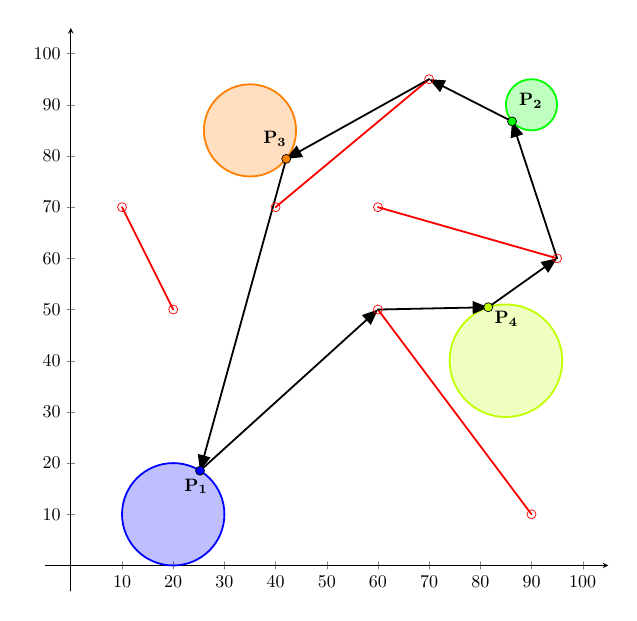
\begin{tikzpicture}[line cap=round,line join=round,>=triangle 45,x=1cm,y=1cm, scale=0.65]
	\begin{axis}[
		x=0.1cm,y=0.1cm,
		axis lines=middle,
		xmin=-5,
		xmax=105,
		ymin=-5,
		ymax=105,
		xtick={-30,-20,...,160},
		ytick={-30,-20,...,95},]
		\clip(-30.537729395742623,-29.679586779798765) rectangle (175.76223117610863,116.68410916363341);
		\draw [line width=1pt,color=ffqqqq] (70,95)-- (40,70);
		\draw [line width=1pt,color=ffqqqq] (95,60)-- (60,70);
		\draw [line width=1pt,color=ffqqqq] (60,50)-- (90,10);
		\draw [line width=1pt,color=ffqqqq] (10,70)-- (20,50);
		\draw [rotate around={0:(20,10)},line width=1pt,color=qqqqff,fill=qqqqff,fill opacity=0.25] (20,10) ellipse (1cm and 1cm);
		\draw [rotate around={0:(90,90)},line width=1pt,color=qqffqq,fill=qqffqq,fill opacity=0.25] (90,90) ellipse (0.5cm and 0.5cm);
		\draw [rotate around={0:(35,85)},line width=1pt,color=ffxfqq,fill=ffxfqq,fill opacity=0.25] (35,85) ellipse (0.9cm and 0.9cm);
		\draw [rotate around={0:(85,40)},line width=1pt,color=bfffqq,fill=bfffqq,fill opacity=0.25] (85,40) ellipse (1.1cm and 1.1cm);
		
		%\draw [->,line width=1pt] (27.07,17.07) -- (40,30);
		%\draw [->,line width=1pt] (40,30) -- (27.07,17.07);
		%\draw [->,line width=1pt] (40,30) -- (40,70);
		%\draw [->,line width=1pt] (40,70) -- (42.19,79.59);
		%\draw [->,line width=1pt] (42.19,79.59) -- (70,95);
		%\draw [->,line width=1pt] (70,95) -- (86.2,86.75);
		%\draw [->,line width=1pt] (86.2,86.75) -- (95,60);
		%\draw [->,line width=1pt] (95,60) -- (81.55,50.45);
		%\draw [->,line width=1pt] (81.55,50.45) -- (60,50);
		%\draw [->,line width=1pt] (60,50) -- (40,30);
		\draw [->,line width=1pt] (42.08,79.44) -- (25.24,18.51);
		\draw [->,line width=1pt] (25.24,18.51) -- (60,50);
		\draw [->,line width=1pt] (60,50) -- (81.55,50.45);
		\draw [->,line width=1pt] (81.55,50.45) -- (95,60);
		\draw [->,line width=1pt] (95,60) -- (86.2,86.75);
		\draw [->,line width=1pt] (86.2,86.75) -- (70,95);
		\draw [->,line width=1pt] (70,95) -- (42.08,79.44);
		
		\draw (20.94789460207184,18.16350179860903) node[anchor=north west] {$\mathbf{P_1}$};
		\draw (86.35454360885365,93.50433831286361) node[anchor=north west] {$\mathbf{P_2}$};
		\draw (36.349175863281,86.08483726584145) node[anchor=north west] {$\mathbf{P_3}$};
		\draw (81.55301964690848,50.8774601568516) node[anchor=north west] {$\mathbf{P_4}$};
		\begin{scriptsize}
			\draw [color=ffqqqq] (70,95) circle (2.5pt);
			\draw [color=ffqqqq] (40,70) circle (2.5pt);
			\draw [color=ffqqqq] (95,60) circle (2.5pt);
			\draw [color=ffqqqq] (60,70) circle (2.5pt);
			\draw [color=ffqqqq] (60,50) circle (2.5pt);
			\draw [color=ffqqqq] (90,10) circle (2.5pt);
			\draw [color=ffqqqq] (10,70) circle (2.5pt);
			\draw [color=ffqqqq] (20,50) circle (2.5pt);
			\draw [fill=qqqqff] (25.24, 18.51) circle (2.5pt);
			\draw [fill=qqffqq] (86.2,86.75) circle (2.5pt);
			\draw [fill=ffxfqq] (42.08,79.44) circle (2.5pt);
			\draw [fill=bfffqq] (81.55,50.45) circle (2.5pt);
		\end{scriptsize}
	\end{axis}
\end{tikzpicture}
\label{fig:solution_tsp}
\end{figure}